\documentclass{article}
\usepackage{amsmath, amssymb, amsthm}
\usepackage{graphicx}
\usepackage{caption}
\usepackage{subcaption}

\graphicspath{ {../images/} }

\title{Removing Projective Distortion from Images}
\author{Mickey Smith}
\date{August 2019}

\begin{document}

\maketitle

\section{Homogenous Coordinates}
Similar to cartesian coordinates, homogenous coordinates are a way to represent points in a given dimension.

\begin{figure}[hbt!]
\centering
\begin{subfigure}{.5\textwidth}
    \centering
    \begin{pmatrix}
        x \\
        y
    \end{pmatrix}
    \caption{Cartesian & $\mathbb{R}^2$}
    \label{fig:coords_sub1}
\end{subfigure}%
\begin{subfigure}{.5\textwidth}
    \centering
    \begin{pmatrix}
        x \\
        y \\
        1
    \end{pmatrix}
    \caption{Homogenous & $\mathbb{R}^2$}
    \label{fig:coords_sub2}
\end{subfigure}
\caption{Representing coordinates as homogenous and cartesian}
\label{fig:coords}
\end{figure}

The only practical difference between cartesian and homogenous for the purposes of this assignment is that homogenous coordinates contain an extra dimension value that represents vector scaling. This allows a point to be further from the origin on its component vector without altering the other coordinates.

\clearpage
\section{Projective Transformations}

\begin{figure}[hbt!]
    \centering
    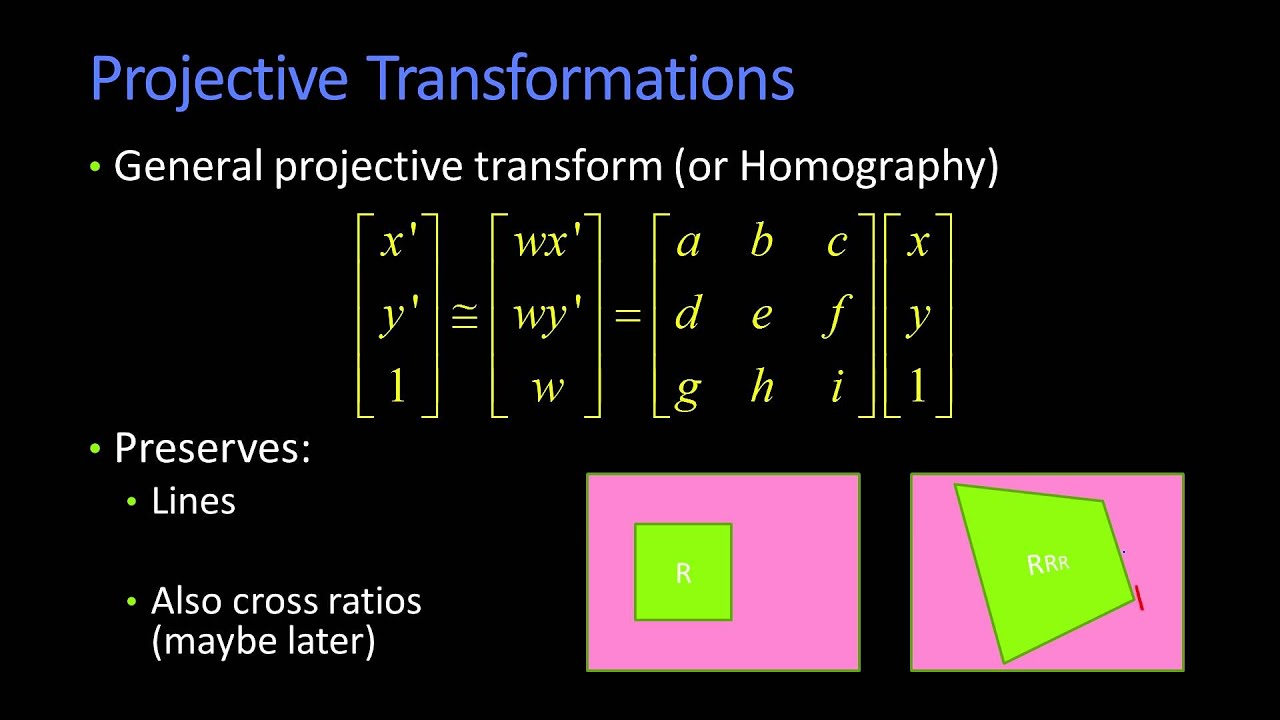
\includegraphics[scale=0.2]{projective_transform}
    \caption{HDSFKJHDF}
\end{figure}

\begin{pmatrix}
    a   &b \\
    c   &d
\end{pmatrix}

\end{document}
